\documentclass[12pt,letterpaper,oneside,reqno]{amsart}
\usepackage{amsfonts}
\usepackage{amsmath}
\usepackage{amssymb}
\usepackage{amsthm}
\usepackage{float}
\usepackage{mathrsfs}
\usepackage{colonequals}
\usepackage[font=small,labelfont=bf]{caption}
\usepackage[left=1in,right=1in,bottom=1in,top=1in]{geometry}
\usepackage[pdfpagelabels,hyperindex,colorlinks=true,linkcolor=blue,urlcolor=magenta,citecolor=green]{hyperref}
\usepackage{graphicx}
\linespread{1.7}
\emergencystretch=1em

\newcommand \anglePower [2]{\langle #1 \rangle \sp{#2}}
\newcommand \bernoulli [2][B] {{#1}\sb{#2}}
\newcommand \curvePower [2]{\{#1\}\sp{#2}}
\newcommand \coeffA [3][A] {{\mathbf{#1}} \sb{#2,#3}}
\newcommand \polynomialP [4][P]{{\mathbf{#1}}\sp{#2} \sb{#3}(#4)}

% ordinary derivatives
\newcommand \derivative [2] {\frac{d}{d #2} #1}                              % 1 - function; 2 - variable;
\newcommand \pderivative [2] {\frac{\partial #1}{\partial #2}}               % 1 - function; 2 - variable;
\newcommand \qderivative [1] {D_{q} #1}                                      % 1 - function
\newcommand \nqderivative [1] {D_{n,q} #1}                                   % 1 - function
\newcommand \qpowerDerivative [1] {\mathcal{D}_q #1}                         % 1 - function;
\newcommand \finiteDifference [1] {\Delta #1}                                % 1 - function;
\newcommand \pTsDerivative [2] {\frac{\partial #1}{\Delta #2}}               % 1 - function; 2 - variable;

% high order derivatives
\newcommand \derivativeHO [3] {\frac{d^{#3}}{d {#2}^{#3}} #1}                % 1 - function; 2 - variable; 3 - order
\newcommand \pderivativeHO [3]{\frac{\partial^{#3}}{\partial {#2}^{#3}} #1}
\newcommand \qderivativeHO [2] {D_{q}^{#2} #1}                               % 1 - function; 2 - order
\newcommand \qpowerDerivativeHO [2] {\mathcal{D}_{q}^{#2} #1}                % 1 - function; 2 - order
\newcommand \finiteDifferenceHO [2] {\Delta^{#2} #1}                         % 1 - function; 2 - order
\newcommand \pTsDerivativeHO [3] {\frac{\partial^{#3}}{\Delta {#2}^{#3}} #1} % 1 - function; 2 - variable;

\newtheorem{thm}{Theorem}[section]
\newtheorem{cor}[thm]{Corollary}
\newtheorem{lem}[thm]{Lemma}
\newtheorem{examp}[thm]{Example}

\numberwithin{equation}{section}

\title[Secure Open ID Connect implementation using Azure]
{Secure Open ID Connect implementation using Azure}
\author[Petro Kolosov]{Petro Kolosov}
\email{kolosovp94@gmail.com}
\keywords{
    Keyword1, Keyword2
}
\urladdr{https://kolosovpetro.github.io}
\subjclass[2010]{26E70, 05A30}
\date{\today}
\hypersetup{
    pdftitle={Secure Open ID Connect implementation using Azure},
    pdfsubject={
        Your Subject List
    },
    pdfauthor={Petro Kolosov},
    pdfkeywords={
        Your Keywords list
    }
}
\begin{document}
    \begin{abstract}
        In this manuscript we discuss the problem of secure storage and transfer of access tokens between microservices.
Web browser may store access tokens both, in local storage or in cookie files.
We propose a secure implementation to store and transfer auth cookies between microservices
using Azure Active Directory, OpenID Connect and ASP .NET Web Framework.
    \end{abstract}

    \maketitle

    \tableofcontents


    \section{Introduction} \label{sec:introduction}
    Your introduction here.
Include some references~\cite{siddiqui2011cross,spett2005cross, bradley2015rfc,hardt2012oauth}.
Lorem Ipsum is simply dummy text of the printing and typesetting industry.
Lorem Ipsum has been the industry's standard dummy text ever since the 1500s, when an unknown printer took a galley
of type and scrambled it to make a type specimen book.
It has survived not only five centuries, but also the leap into electronic typesetting, remaining essentially unchanged.
It was popularised in the 1960s with the release of Letraset sheets containing Lorem Ipsum passages, and more
recently with desktop publishing software like Aldus PageMaker including versions of Lorem Ipsum.

OAuth 2.0 flow diagram
\begin{figure}[H]
    \centering
    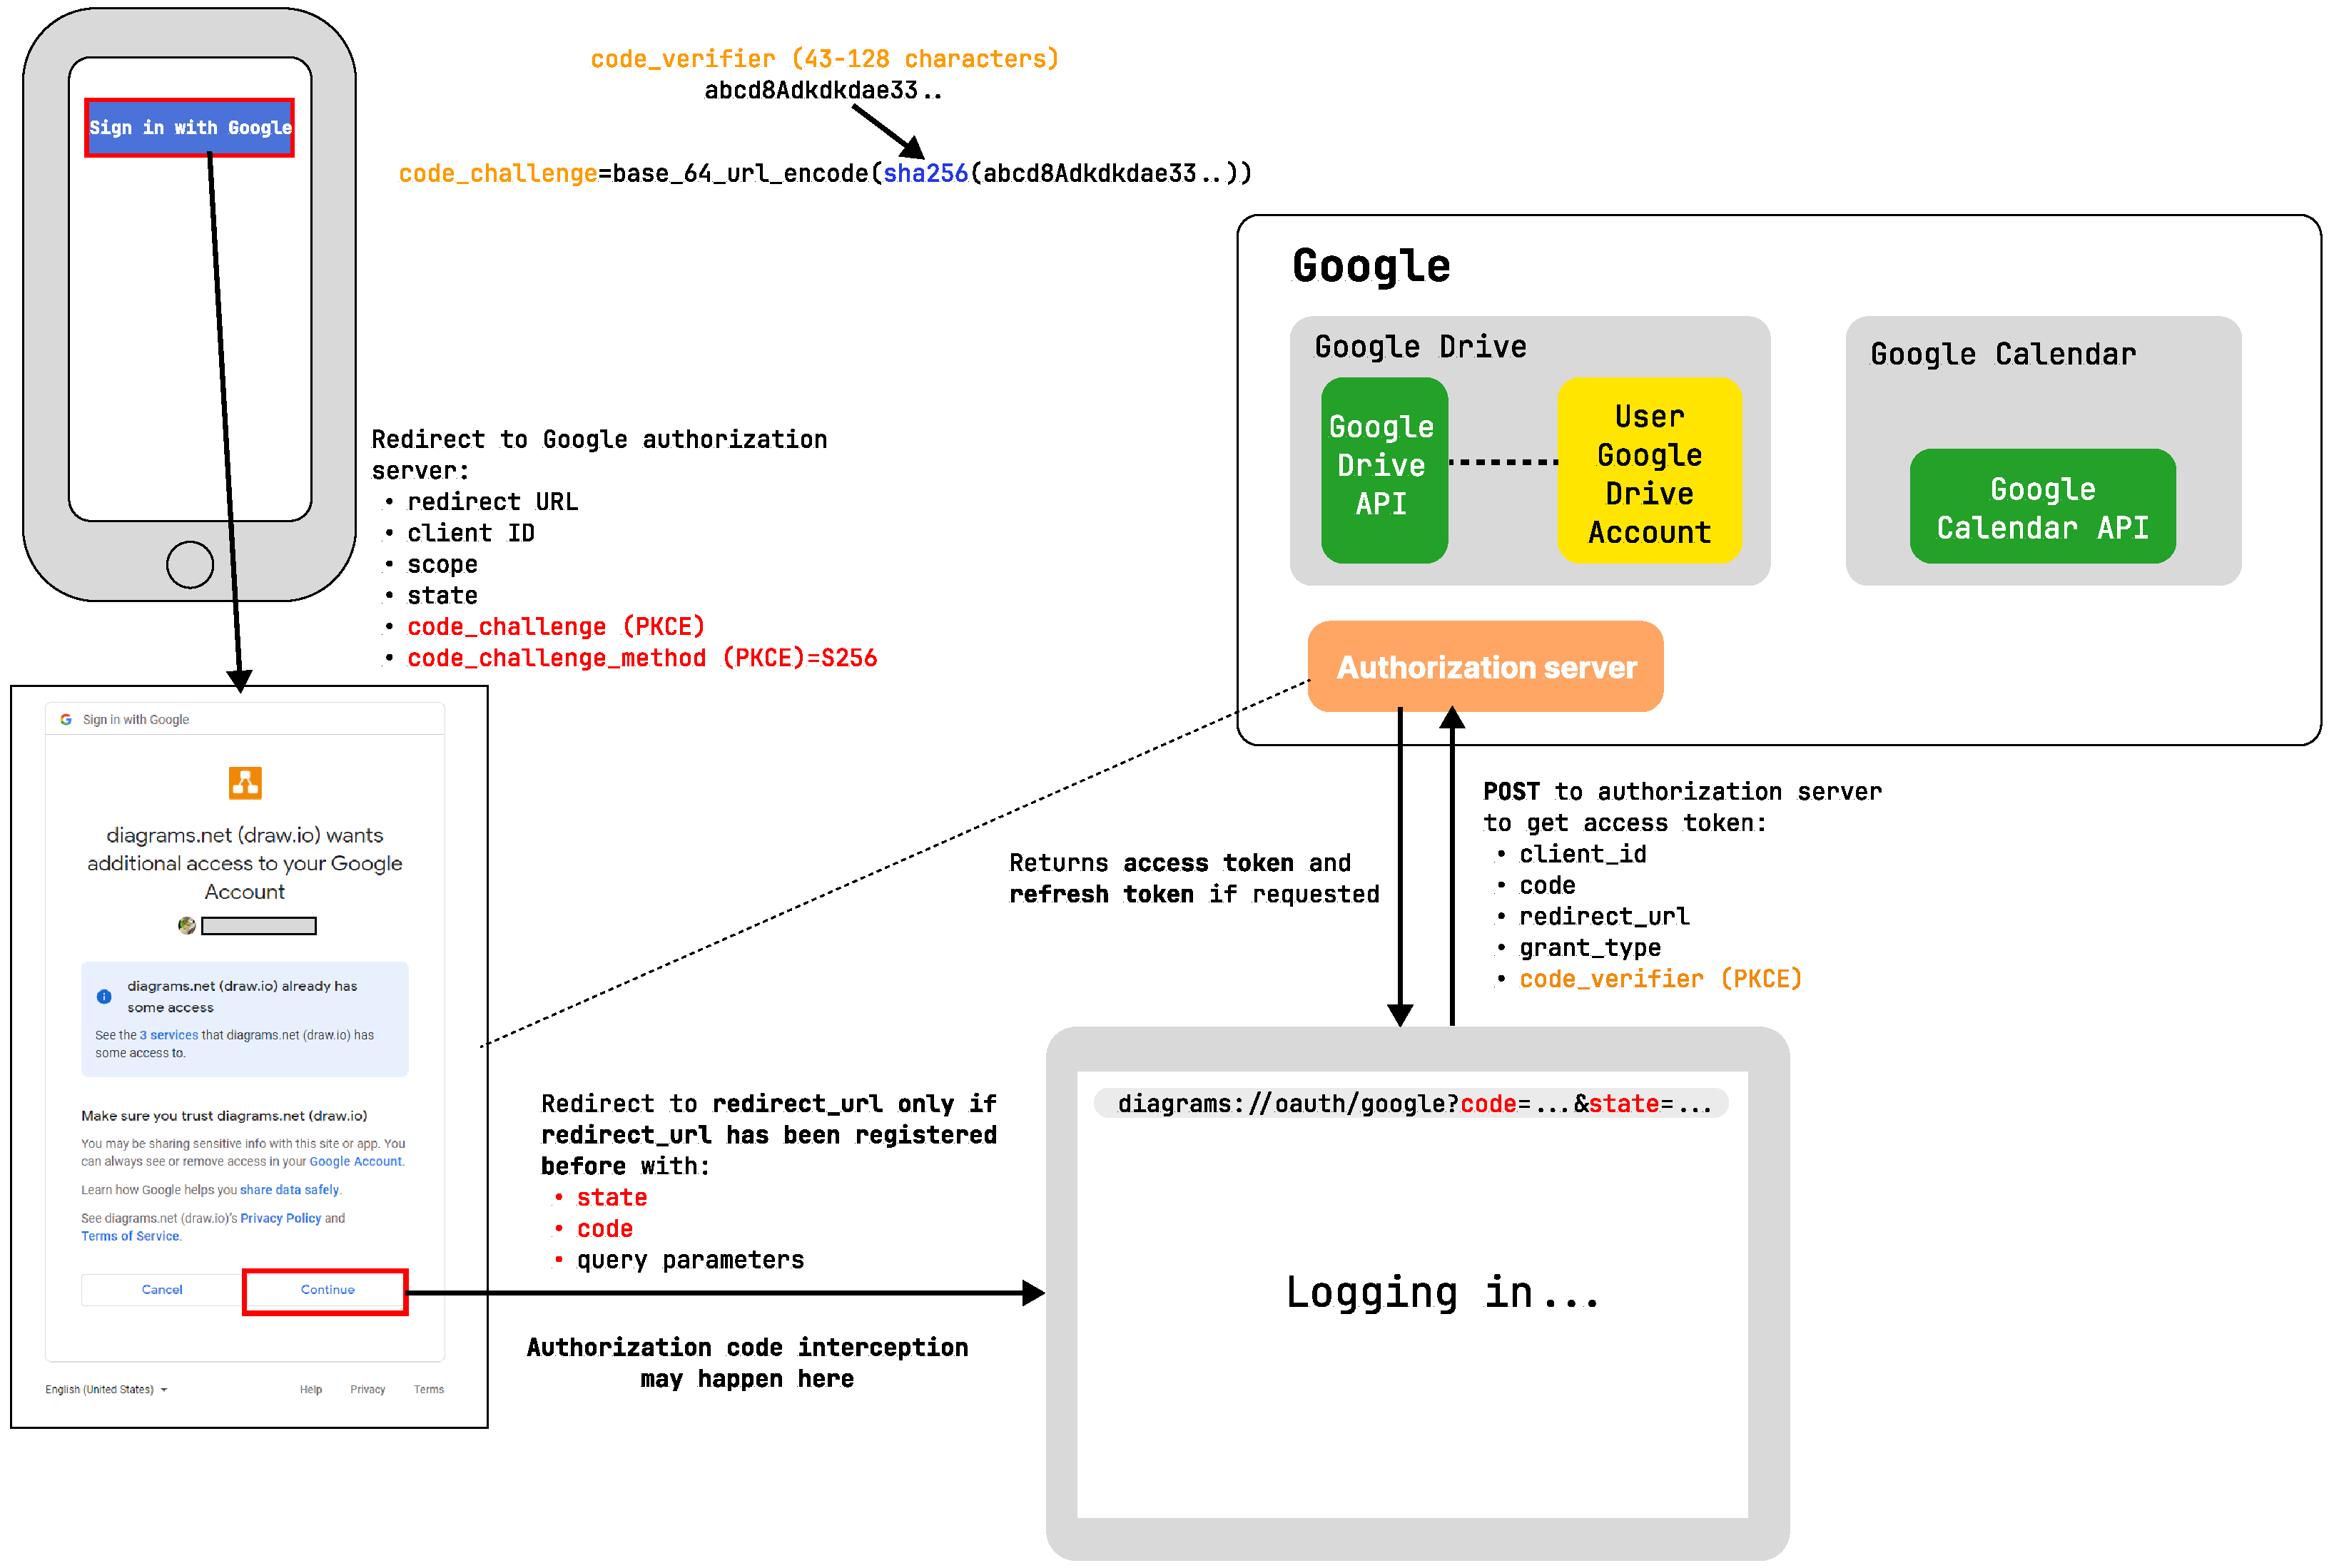
\includegraphics[width=1\textwidth]{img/OAuthPkceScheme_1570_1055}
    ~\caption{OAuth 2.0 with PKCE flow diagram.}\label{fig:oauth_with_pkce}
\end{figure}


    \section{Conclusions}\label{sec:conclusions}
    In this manuscript we explore the problem of secure storage and transfer of access tokens between microservices.
Particular attention was paid to possible vulnerabilities during transfer of access tokens such
as Cross-Site Scripting (XSS) and Cross-Site Request Forgery (CSRF).

To eliminate these vulnerabilities, it is necessary to store authorization tokens in cookies with mandatory
\texttt{HttpOnly} and \texttt{SameSite} settings such that \texttt{SameSite} values should be \texttt{Lax} or \texttt{Strict}.
Therefore, cookies are either transmitted via secure \texttt{HTTP} methods or not transmitted at all.

User authentication to be implemented using the OIDC protocol~\cite{siriwardenaOpenid2020, sakimuraOpenid2014}
in couple with Authorization code flow with PKCE~\cite{bradley2015rfc}.
The main principle of the OIDC protocol is described more detailed in Chapter 2.

Also, we provide an authentication / authorization implementation based on the ASP.NET Core Web API backend and Angular
frontend application.
These apps are stored under single domain to eliminate necessity to transfer authorization cookies cross domain way.
The transfer of access tokens to microservices is implemented using Reverse Proxy YARP~\cite{microsoftYarp2021} so that
the access token is automatically substituted in the request header.

In addition, we proposed a mechanism to refresh an access token through the Ticket Store~\cite{microsoftIticketstore2023} entity
and Hosted Service~\cite{microsoftHostedservice2023}.
Therefore, the Ticket Store checks each request for access token expiration.
In case of expiration of the access token, the access token is refreshed by means of authorization microservice.
Ticket store also stores the pair of the access and refresh token inside \texttt{AuthenticationTicket} entity~\cite{microsoftAuthenticationTicket2023}.

Finally, in this manuscript we proposed a solution to the problem of securely storing an access token and passing it between microservices,
eliminating the Cross-Site Scripting (XSS) and Cross-Site Request Forgery (CSRF) vulnerabilities.

    \bibliographystyle{unsrt}
    \bibliography{SecureAzureOIDCReferences}

\end{document}
